
\begin{figure*}[ht!]
    \centering
    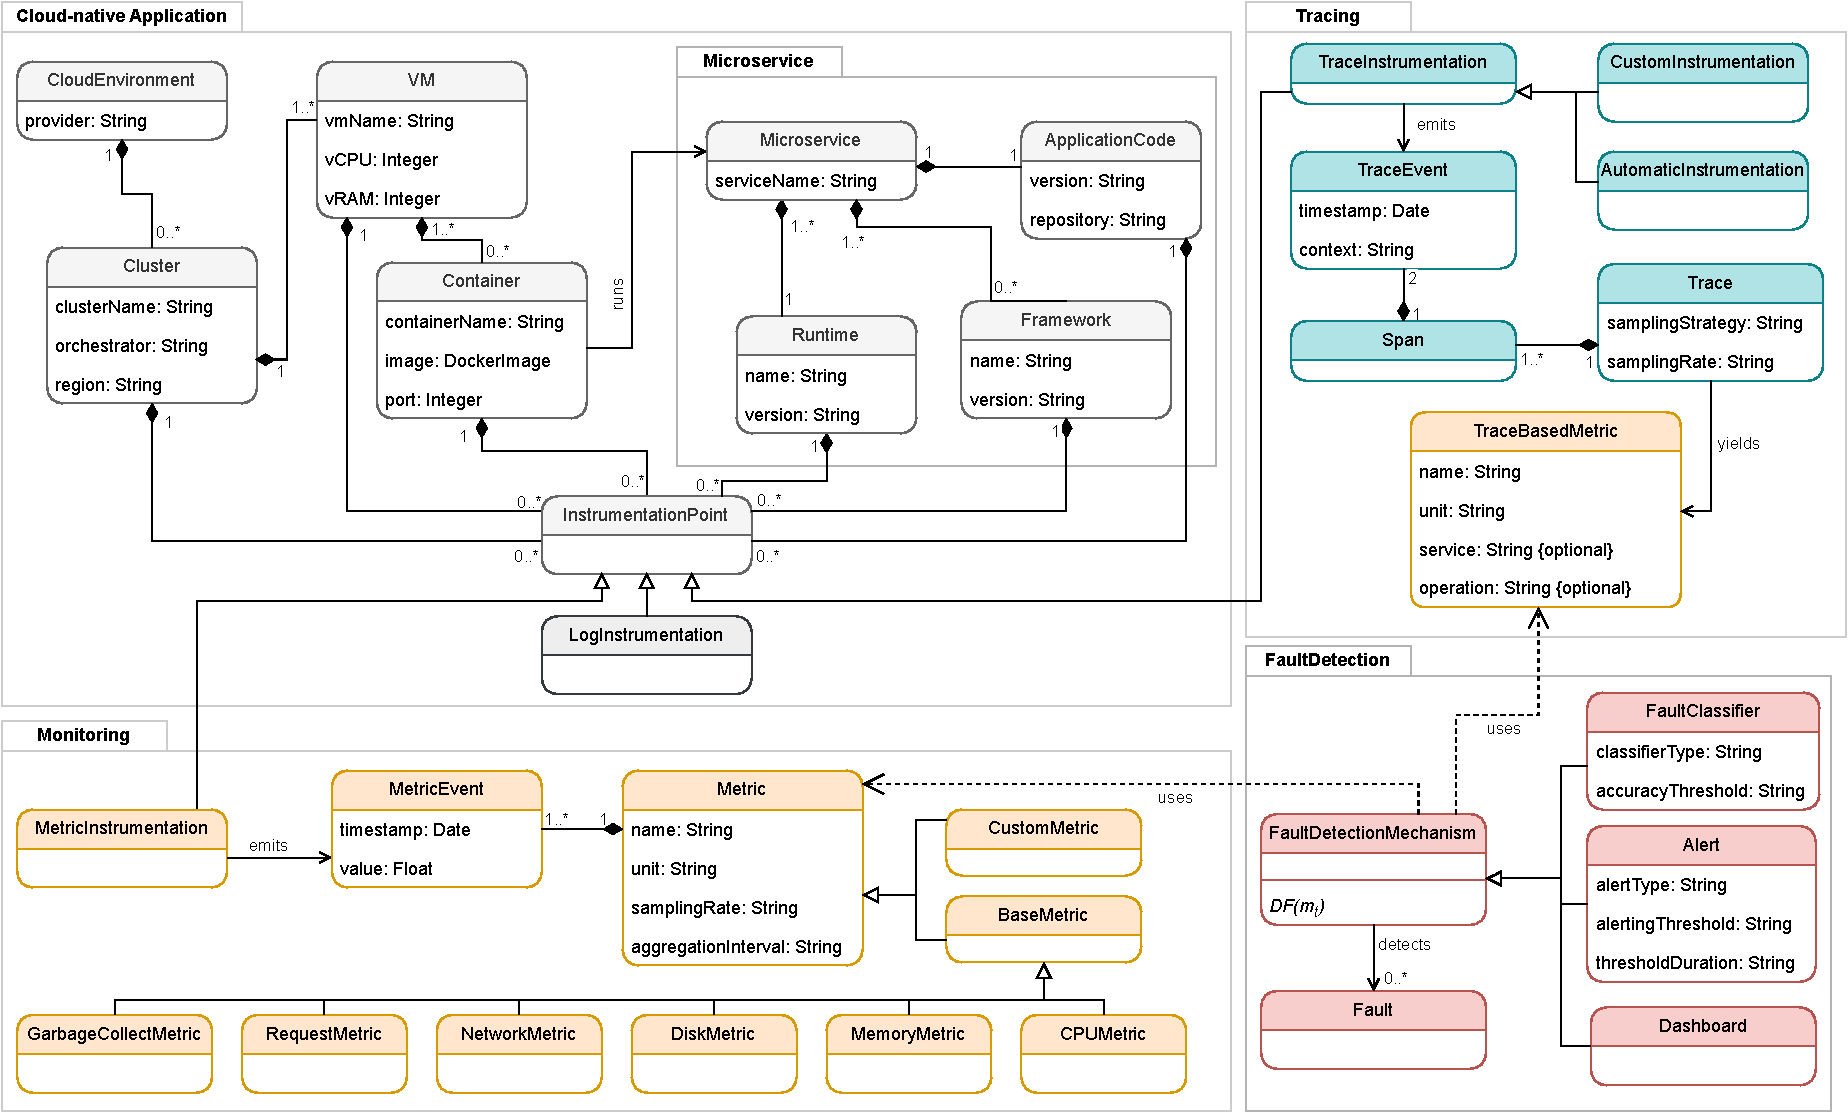
\includegraphics[width=\textwidth]{figures/model_v9.pdf}
    \caption{Model of Observability Design Decisions in Cloud-Native Applications}
    \label{fig:model}
\end{figure*}
Ensuring the reliable operation of microservice-based applications is a complicated task that requires observability. Observability, as defined in literature, is the ability to measure the internal state of a system by its outputs \cite{Niedermaier_ObservabilityInterviewStudy_2019}. The process of defining these outputs is what we define as ``observability design decisions". 
In this section, we delve into the intricacies and nuances of these decisions by modeling a typical cloud-native microservice application deployed in accordance with modern practices. 
With this model, we aim to show the scale and scope of observability design decisions, plus it will serve as a common language for practitioners to understand and discuss observability design alternatives. Figure \ref{fig:model} shows our model, which we break down in the following paragraphs.

A \textbf{Cloud-native Application} is deployed in a \models{Cloud Environment} managed by a third-party provider. The model represents the application topology as one or more deployment clusters (\models{Cluster}), deployed in a specific region and managed by an orchestrator. The orchestrator is a deployment technology, e.g. Kubernetes\footnote{\url{https://kubernetes.io}} or Docker Compose\footnote{\url{https://docs.docker.com/compose/}}, that automates the deployment and management of \models{Containers} across virtual machines (\models{VMs}). Each container runs an instance of a \models{Microservice}. We model a microservice as a composition of a \models{Runtime}, which provides the language-specific environment of the microservice, e.g. the Java Runtime. Microservices can also be composed of a number of \models{Frameworks}, which offer reusable components that streamline the development process, e.g., Django or gRPC. Lastly, microservices are also composed of the \models{Application Code} written by the development team.

In order to capture observability data, a cloud-native application needs to be instrumented through so-called \models{InstrumentationPoints}. Instrumentation refers to the process of embedding code within a software component that enables it to collect and emit metrics, traces and logs. Some components of the cloud-native deployment stack are equipped with so-called automatic instrumentation, meaning that instrumentation points are provided out-of-the-box. Depending on the observability data they collect, \models{InstrumentationPoints} can be of type \models{MetricInstrumentation}, \models{LogInstrumentation} and \models{TraceInstrumentation}. Each instrumentation type supports a different observability practice. 
While logging is similarly important for building reliable software systems, we mainly focus on modeling monitoring and tracing in this, as logging is less standardized to make a generic model beyond timestamped, human-readable text messages.

\textbf{Monitoring} is the continuous measurement of quantitative properties of a system over a period of time. \texttt{MetricInstrumentation}-Points emit \texttt{MetricEvents} which are timestamped value measurements. A \texttt{Metric}, in turn, represents the time-series collection of several \texttt{MetricEvents}. They may be simple \texttt{BaseMetrics}, collected directly through automatic instrumentation points provided in \texttt{Clusters}, \texttt{VMs}, \texttt{Containers}, \texttt{Runtimes} and \texttt{Frameworks}. In Figure \ref{fig:model} we show several of these types of \texttt{BaseMetrics}, but the list is not intended to be exhaustive. \texttt{Metrics} may also be specified and instrumented by developers in the case of \texttt{CustomMetrics}. While designing the monitoring of an application, practitioners face several design decisions, including (1) what \texttt{BaseMetrics} to collect from the available automatic \texttt{InstrumentationPoints}, (2) whether to add \texttt{CustomMetrics} and if yes, where to add the \texttt{InstrumentationPoints}, (3) how to configure the attributes \texttt{samplingRate} and \texttt{aggregationInterval} for each \texttt{Metric} instance.


\textbf{Tracing} enables end-to-end observation of appli\-cation behaviour by retrieving
and aggregating event data in so-called traces. In this context, a \models{TracingInstrumentation}-Point, which can be of type \models{AutomaticInstrumentation} if supported natively by the microservice \models{Runtime} or \models{Framework}, or of type \models{CustomInstrumentation} if added to the \models{ApplicationCode} by the development team, emits a \models{TraceEvent}. A pair of \models{TraceEvents} demarcating entry and exit build a \models{Span}, and multiple spans form a \models{Trace}. The information inside traces can further be processed into \models{TraceBasedMetrics}, e.g. the duration of spans or of entire traces. While designing the tracing of an application, practitioners again face several design decisions, namely (1) where to add \models{CustomInstrumentation} and (2) how to configure the attributes \models{samplingStrategy} and \models{samplingRate}.

For \textbf{Fault Detection}, observability systems employ so-called \models{FaultDetectionMechanisms} to be able to detect \models{Faults}. These mechanisms can employ a variety of detection methods, including pre-trained \models{Classifiers}, \models{Alerts},  or by having an trained site-reliability engineers look at \models{Dashboards}. For fault detection, practitioners first (1) need to select a feasible \models{FaultDetectionMechanism}, then (2) set appropriate attributes to not overload reliability teams and yet provide fast response to potential failures. Naturally, the prior design decisions on logging, monitoring and tracing strongly influence the quality of these detection methods, as too few inputs may lead to a low sensitivity, and too many observations lead to too much noise and thus may lead to oversensitivity.
